\chapter{Organisation d'un document}
\label{chap:organisation}


\section{Choix d'une classe}
\label{sec:organisation:classe}

La toute première chose à faire au moment de se lancer dans la
rédaction d'un document avec {\LaTeX} consiste normalement à choisir
une classe pour celui-ci. Nous avons déjà expliqué à la
\autoref{sec:bases:classes} comment spécifier la classe à utiliser. La
présente section présente les différences entre les classes ainsi que
les principales options disponibles.

Les classes standards sont \class{article}, \class{report},
\class{book}, \class{letter} et \class{slides}.

\begin{description}
\item[\normalfont\class{article}] Articles scientifiques et autres
  documents de longueur modérée ne nécessitant pas une mise en page
  élaborée. Le folio (numéro de page) est placé au centre du pied de
  page. Le titre apparait dans le haut de la première page,
  immédiatement suivi du texte.
\item[\normalfont\class{report}] Rapports et autres documents plus
  longs pouvant être divisés en chapitres. Le titre apparait sur une
  page de titre. La mise en page est autrement identique à celle de la
  classe \class{article}.
\item[\normalfont\class{book}] Longs documents divisés en chapitres.
  La mise en page est conçue pour une impression recto-verso. L'entête
  de la page (autre que la première du chapitre) contient le folio sur
  le bord extérieur et le titre de chapitre (page paire) ou le titre
  de section (page impaire). Le titre apparait sur une page de titre.
\item[\normalfont\class{letter}] Lettres et correspondance. Bien que
  puissante, cette classe est plus rarement utilisée. Nous n'en traitons
  pas davantage dans ce document.
\item[\normalfont\class{slides}] Diapositives simples pour des
  présentations. La \autoref{sec:trucs:diapositives} traite plus en
  détail de la production de diapositives.
\end{description}

On trouvera un sommaire des principales caractéristiques des classes
\class{article}, \class{report} et \class{book} dans le
\autoref{tab:organisation:classes}. De plus, les figures
\ref{fig:organisation:classes:article}--\ref{fig:organisation:classes:book}
fournissent des exemples de mise en page pour ces trois classes.

\begin{table}
  \caption{Caractéristiques des principales classes standards}
  \label{tab:organisation:classes}
  \begin{tabularx}{1.0\linewidth}{XXXXX}
    \toprule
    Classe & Divisions & Disposition & Entête & Pied de page \\
    \midrule
    \class{article} & parties,\newline sections, \dots
                       & recto & vide & folio centré \\
    \addlinespace[6pt]
    \class{report} & parties,\newline chapitres,\newline sections, \dots
                       & recto & vide & folio centré \\
    \addlinespace[6pt]
    \class{book} & parties,\newline chapitres,\newline sections, \dots
                       & recto-verso & folio, titres & vide \\
    \bottomrule
  \end{tabularx}
\end{table}

\begin{figure}
  \begin{minipage}{0.48\linewidth}
    \fbox{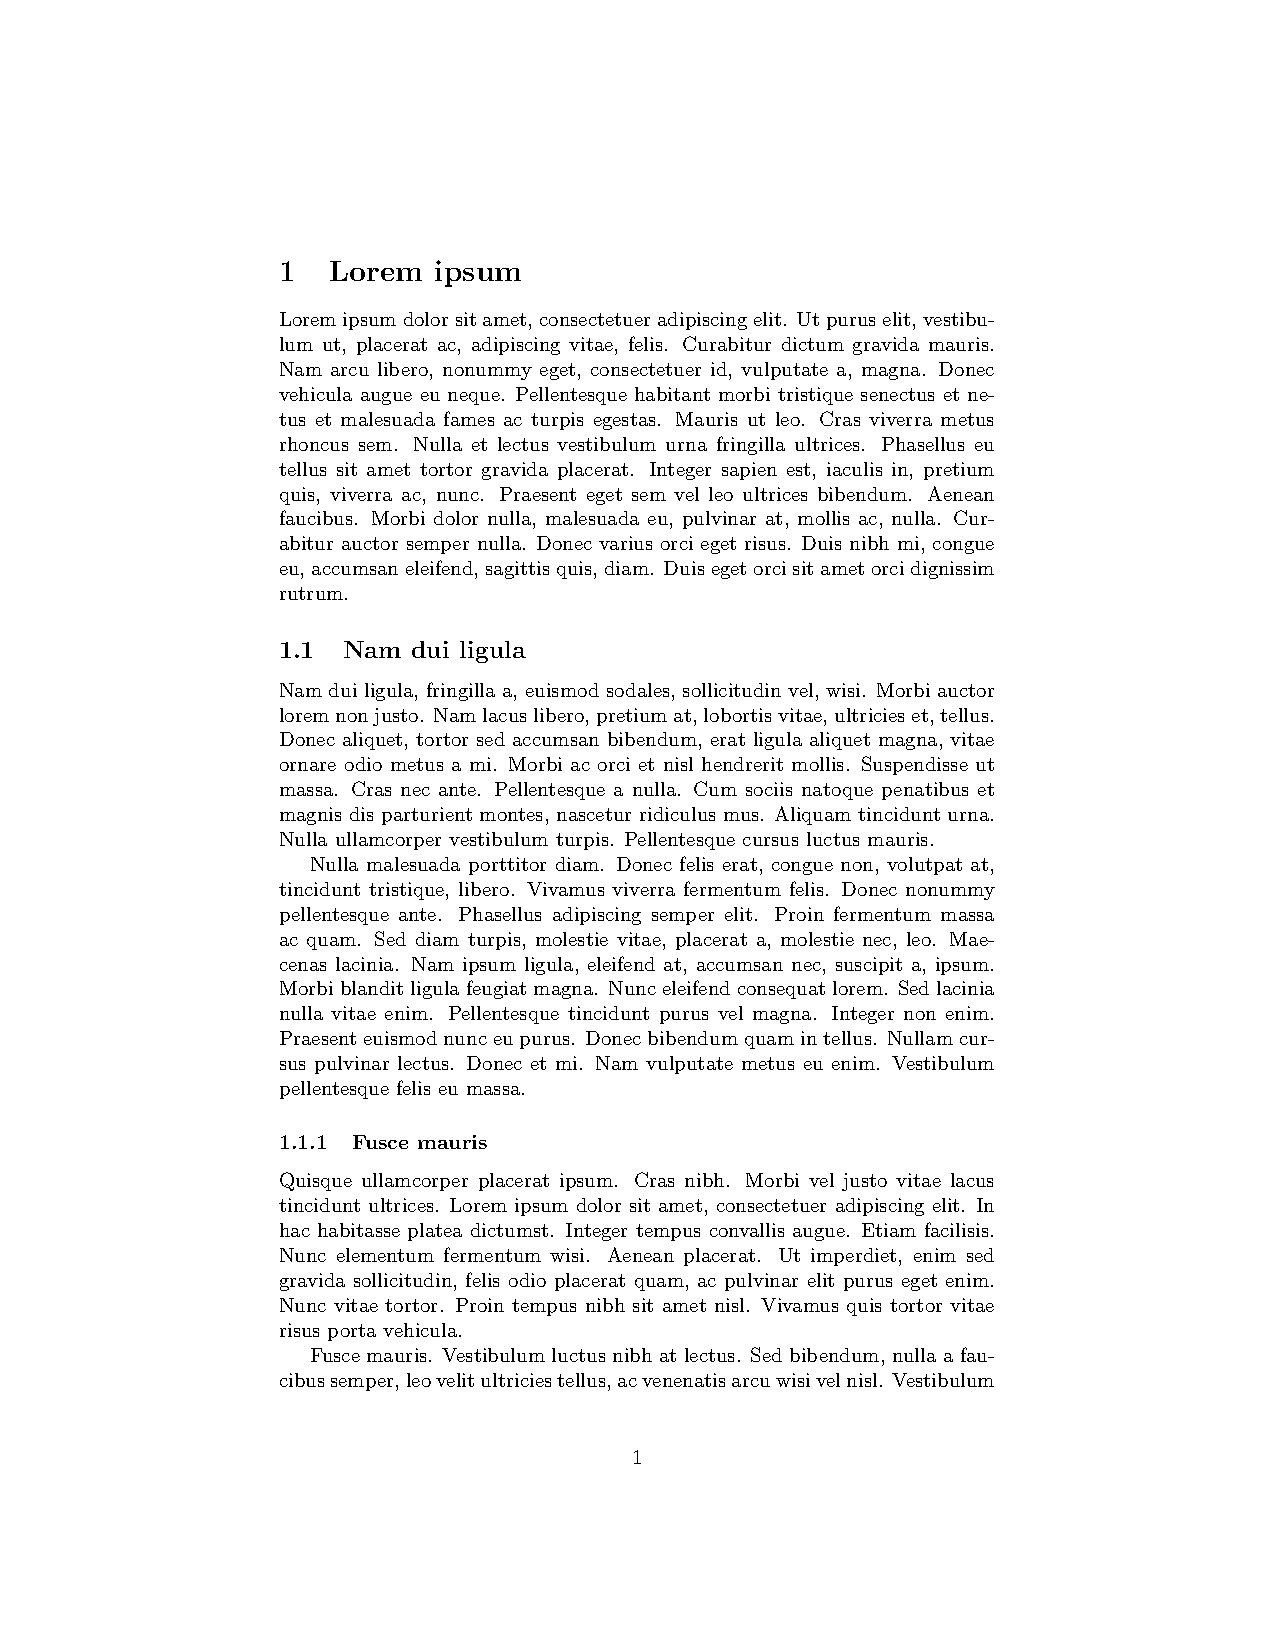
\includegraphics[page=1,width=\linewidth]{exemple-classe-article}}
  \end{minipage}
  \hfill
  \begin{minipage}{0.48\linewidth}
    \fbox{\includegraphics[page=2,width=\linewidth]{exemple-classe-article}}
  \end{minipage}
  \caption{Exemple de mise en page avec la classe \class{article}}
  \label{fig:organisation:classes:article}
\end{figure}

\begin{figure}
  \begin{minipage}{0.48\linewidth}
    \fbox{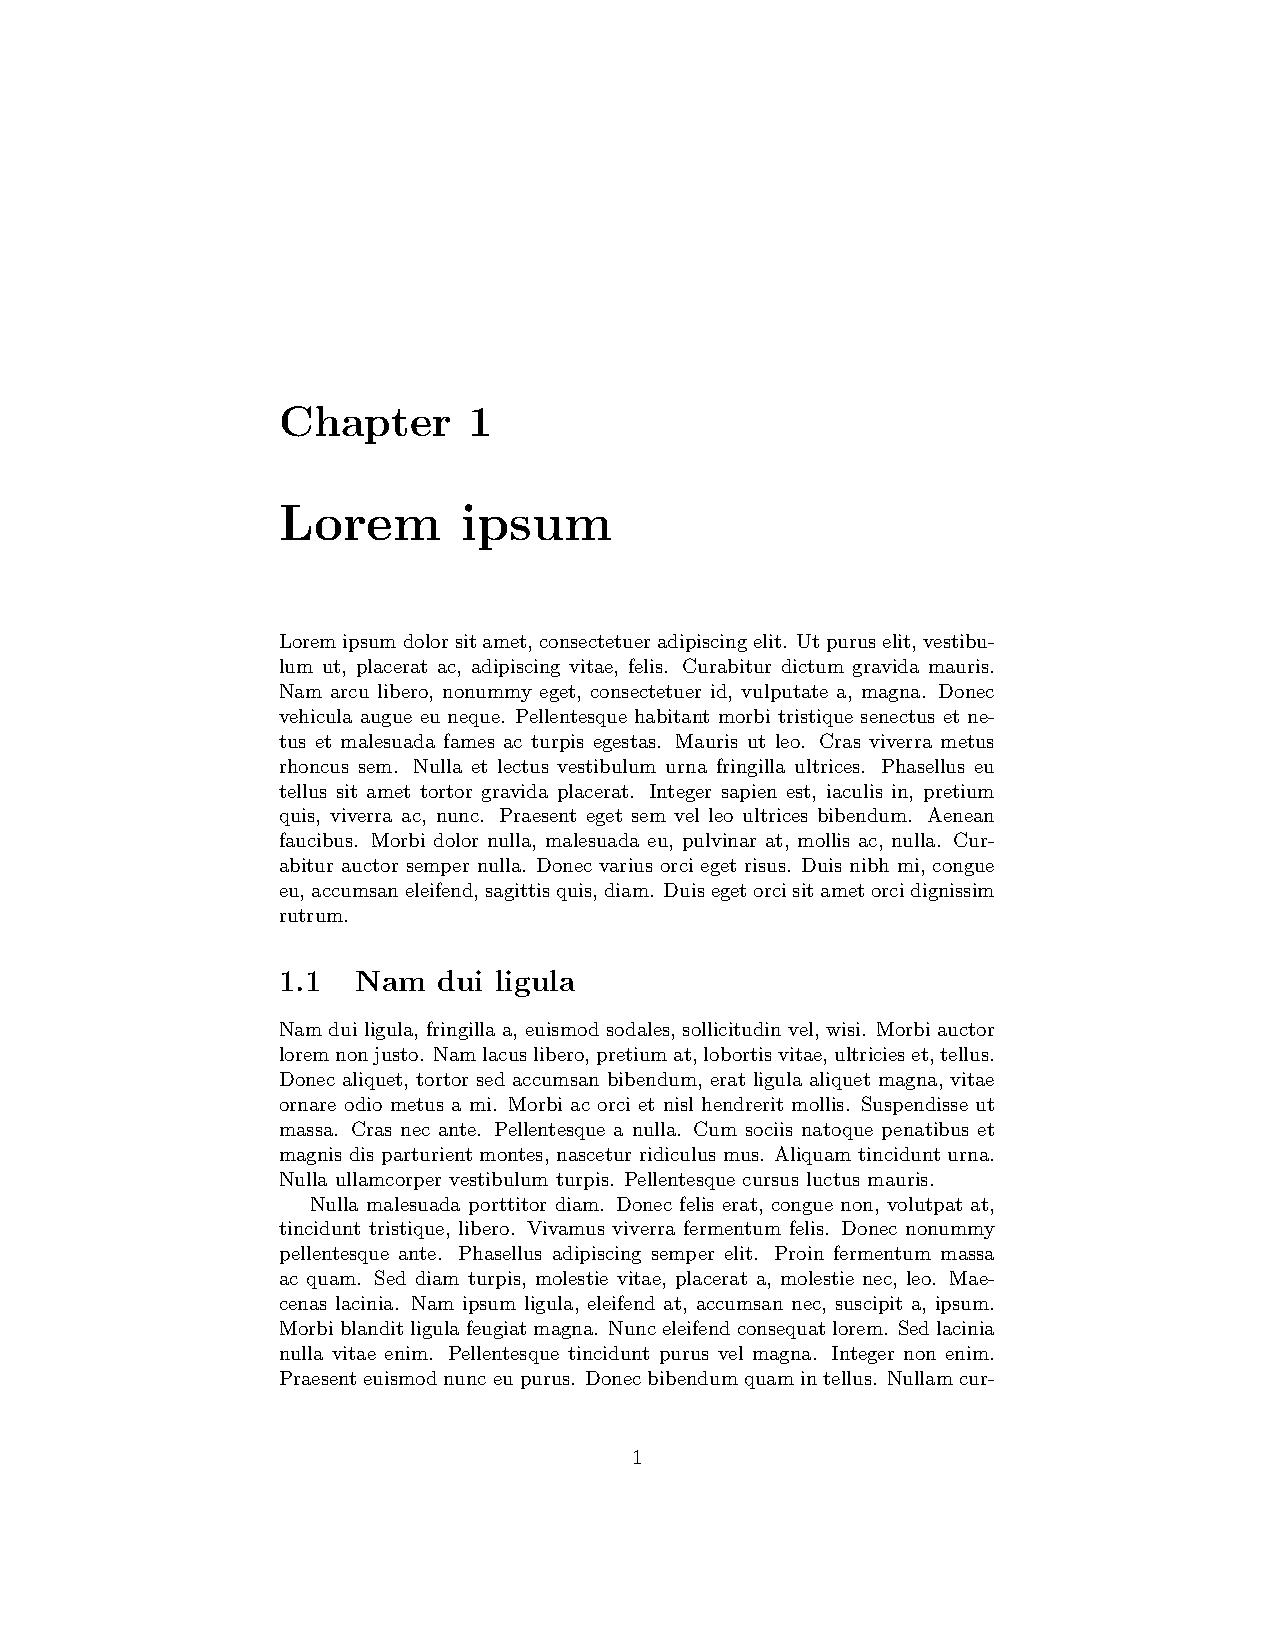
\includegraphics[page=1,width=\linewidth]{exemple-classe-report}}
  \end{minipage}
  \hfill
  \begin{minipage}{0.48\linewidth}
    \fbox{\includegraphics[page=2,width=\linewidth]{exemple-classe-report}}
  \end{minipage}
  \caption{Exemple de mise en page avec la classe \class{report}}
  \label{fig:organisation:classes:report}
\end{figure}

\begin{figure}
  \begin{minipage}{0.48\linewidth}
    \fbox{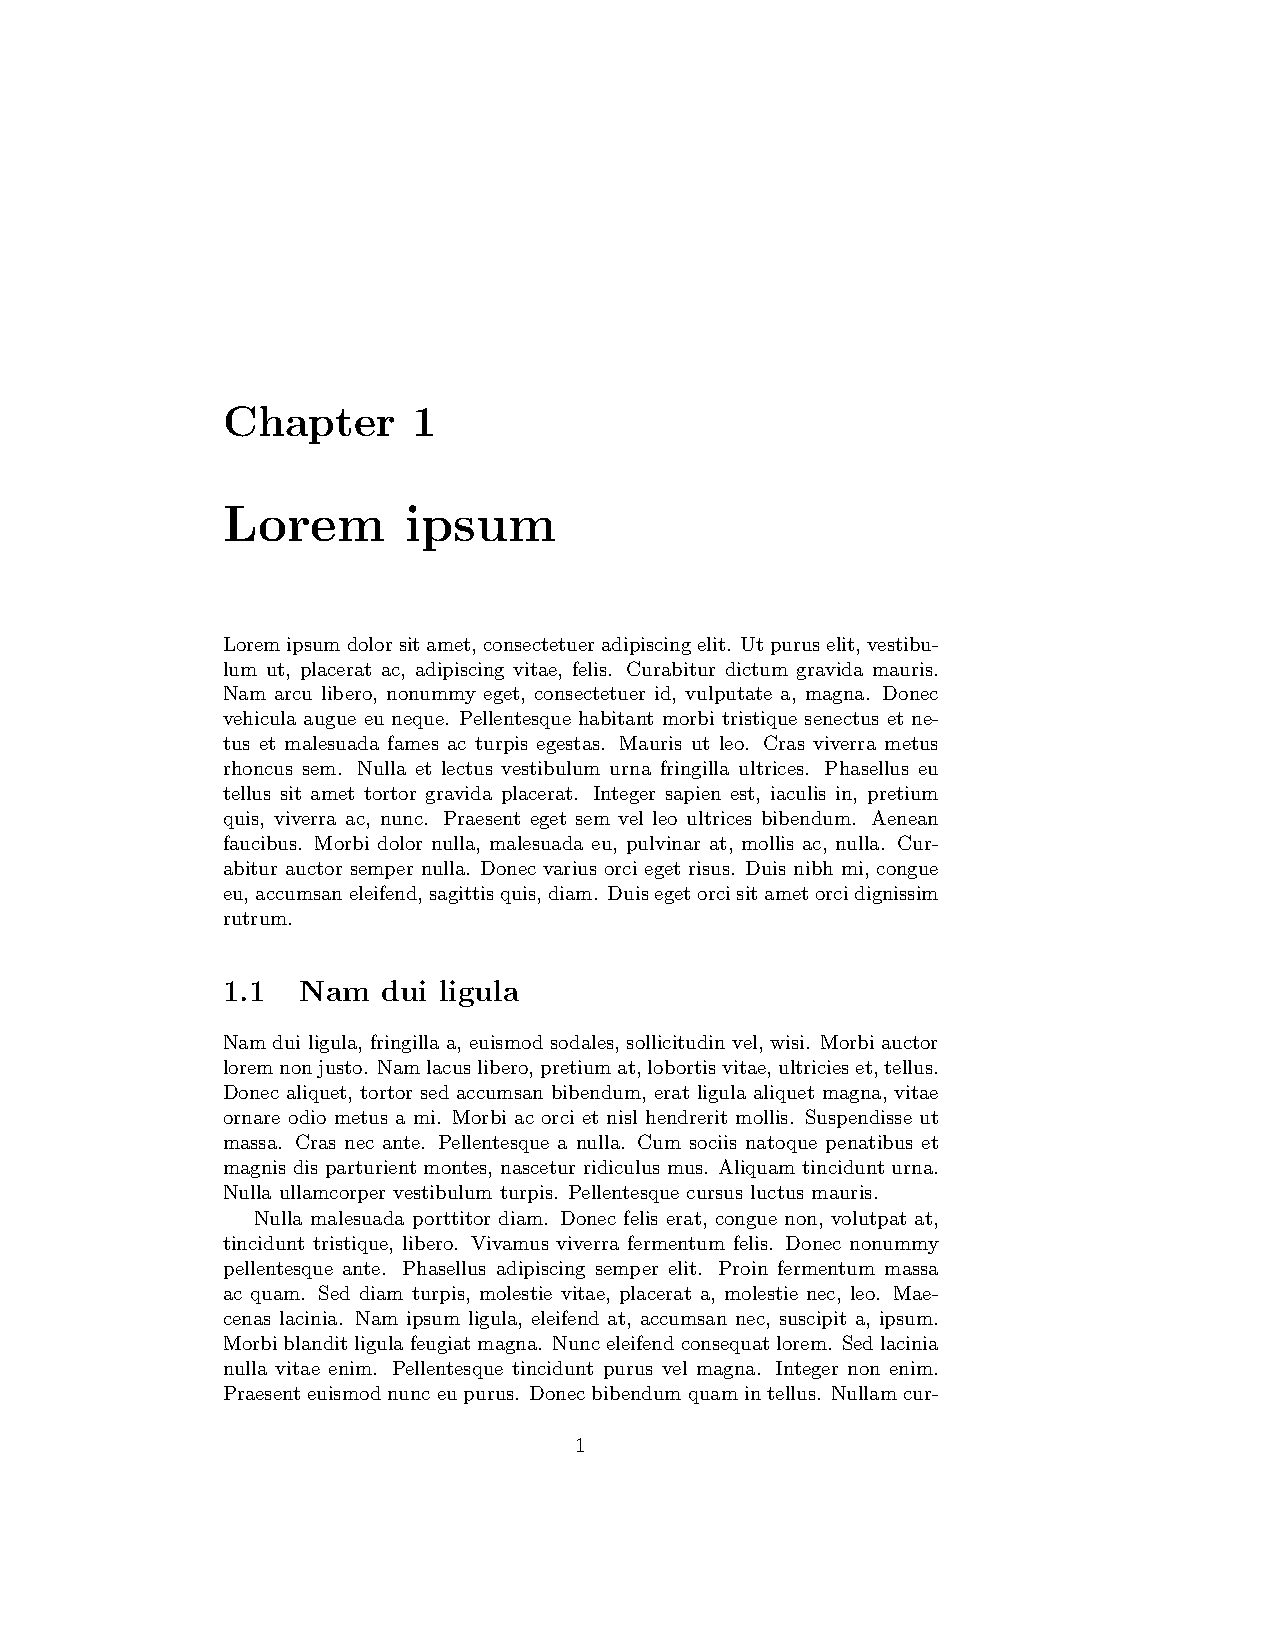
\includegraphics[page=1,width=\linewidth]{exemple-classe-book}}
  \end{minipage}
  \hfill
  \begin{minipage}{0.48\linewidth}
    \fbox{\includegraphics[page=2,width=\linewidth]{exemple-classe-book}}
  \end{minipage}
  \caption{Exemple de mise en page avec la classe \class{book}}
  \label{fig:organisation:classes:book}
\end{figure}

Ce document fait une large place à la classe \class{memoir}
\citep{memoir}, une extension de la classe standard \class{book} qui
facilite à plusieurs égards la préparation de documents d'allure
professionnelle dans {\LaTeX}. Nous recommandons d'utiliser cette
classe en lieu et place de la classe \class{book}, ou même de la
classe \class{article} (voir ci-dessous).

La classe \class{memoir} est très configurable et elle incorpore
d'office plus de 30 des paquetages les plus populaires\footnote{%
  Consulter la section~18.24 de la documentation de \class{memoir}
  pour la liste ou encore le fichier journal (\emph{log}) de la
  compilation d'un document utilisant la classe.}. %
Comme la classe fait partie des distributions {\LaTeX} modernes, elle
devrait être installée et disponible sur votre système. Elle est
livrée avec une %
\doc{memman}{http://texdoc.net/pkg/memoir} %
exhaustive: le manuel d'instructions fait près de 600~pages! Il peut
être utile de s'y référer de temps à autre pour réaliser une mise en
page particulière.

Les auteurs d'un mémoire ou d'une thèse déposé à l'Université Laval
doivent utiliser la classe \class{ulthese} \citep{ulthese}. Celle-ci
est basée sur la classe \class{memoir}. Par conséquent, toutes les
fonctionnalités de \class{memoir} se retrouvent dans \class{ulthese}.

On rappelle que l'on charge une classe de document au début du
préambule avec la commande
\begin{lstlisting}
\documentclass`\oarg{options}\marg{classe}'
\end{lstlisting}
Les \meta{options} disponibles varient d'une classe à l'autre. Les
plus courantes sont les suivantes.
\begin{description}
\item[\mdseries \code{10pt}, \code{11pt}, \code{12pt}] Taille de la
  police du document en points. La valeur par défaut est \code{10pt}.
  Nous recommandons d'utiliser plutôt \code{11pt}. C'est la taille par
  défaut avec la classe \class{ulthese}.
\item[\mdseries \code{oneside}, \code{twoside}] Disposition du
  document en recto seulement ou en recto-verso. Ces options ne sont
  utiles que pour modifier la disposition par défaut de la classe. Les
  thèses et mémoire de l'Université Laval sont produits en recto
  seulement.
\item[\mdseries \code{openright}, \code{openany}] Position de la
  première page des chapitres toujours à droite (page impaire) ou
  immédiatement après la dernière page du chapitre précédent. Avec la
  valeur par défaut, \code{openany}, {\LaTeX} insérera une page
  blanche dans le document si un chapitre se termine sur une page
  impaire.
\item[\mdseries \code{article} (classe \class{memoir} seulement)] Mise
  en page comme celle d'un article. Avec cette option, \class{memoir}
  peut remplacer la classe \class{article}, ce qui permet d'utiliser
  une seule et même classe pour les deux principaux types de document
  (article et livre).
\end{description}

D'autres options permettent de contrôler la position du titre, la
disposition en une ou deux colonnes, ou encore la position des
équations hors paragraphe. \citet{Thurnherr:class-options} offre une
présentation succincte des options standards. Le chapitre~1 de la %
\doc{memman}{http://texdoc.net/pkg/memoir} %
de \class{memoir} traite en plus des ajouts propres à la classe.



\section{Parties d'un document}

Tout document de plus de quelques pages est normalement divisé en
chapitres, sections, sous-sections, etc. Il peut comporter une ou
plusieurs annexes et débuter par un résumé, notamment s'il s'agit d'un
article scientifique. Le document est habituellement coiffé d'un
titre, mais celui-ci est parfois affiché sur une page de titre
séparée.

Toutes ces considérations relevant essentiellement de la mise en page,
{\LaTeX} s'en charge pour nous. L'auteur n'a qu'à spécifier la
strucure logique du document à l'aide des commandes de la présente
section.

\subsection{Titre et page de titre}
\label{sec:organisation:parties:titre}

{\LaTeX} rend très simple la composition du titre d'un article
scientifique ou d'une page de titre simple (classes \class{report},
\class{book}, \class{memoir}). En premier lieu, on spécifie,
habituellement dans le préambule, le titre du document, le nom du ou
des auteurs et la date de publication avec les commandes suivantes:
\begin{lstlisting}
\title`\marg{Titre du document}'
\author`\marg{Prénom Nom {\bs\bs} Affiliation {\bs\bs} Adresse}'
\date`\marg{Date ou autre texte}'
\end{lstlisting}
Un long titre sera scindé automatiquement. L'auteur peut aussi scinder
le titre manuellement en insérant la commande {\bs\bs} aux points de
coupure. %
Si l'ouvrage comporte deux auteurs ou plus, on insère les informations
dans la commande \cmd{\author} les unes après les autres en séparant
chaque entrée par la commande \cmdprint{\and}. %
La commande \cmd{\date} insère le texte donné en argument (qu'il
s'agisse d'une date ou non) à l'endroit prévu à cet effet par
{\LaTeX}. Si l'on omet la commande, {\LaTeX} insère la date du jour au
moment de la compilation. Pour ne pas afficher la date, on laisse
l'argument vide:
\begin{lstlisting}
\date{}
\end{lstlisting}

Dans les articles scientifiques, le nom d'un auteur est fréquemment
suivi d'un appel de note renvoyant à des remerciements à un organisme
subventionnaire ou à quelque autre information additionnelle sur
l'auteur. On insère une telle note et son appel à l'endroit approprié
dans les commandes \cmd{\title} ou \cmd{\author} avec la commande
\begin{lstlisting}
\thanks`\marg{Texte}'
\end{lstlisting}

Les commandes ci-dessus ne permettent que de saisir les informations
relatives au titre. Pour produire le titre il faut, en second lieu,
insérér dans le corps du document la commande
\begin{lstlisting}
\maketitle
\end{lstlisting}

\begin{exemple}
  \label{ex:organisation:titre}
  Le code ci-dessous permet de créer un titre d'article standard. La
  page composée avec {\XeLaTeX} (puisque nous utilisons le paquetage
  \pkg{fontspec}) se trouve à la \autoref{fig:organisation:titre}.
  \begin{demo}
    \lstinputlisting[lastline=19]{exemple-titre.tex}
  \end{demo}

  La date de publication apparaissant dans l'illustration de la
  \autoref*{fig:organisation:titre} est celle de la compilation
  puisque la commande \cmdprint{\date} n'apparait pas dans le code
  source.

  On remarquera également que nous avons placé un symbole de
  commentaire \% immédiatement après le nom de l'auteur dans le code
  source. Tel qu'expliqué à la \ref{sec:bases::caracteres:espaces},
  c'est pour éviter que {\LaTeX} transforme le retour à la ligne avant
  la commande \cmd{\thanks} en une espace entre le nom et l'appel de
  note.

  (Le paquetage \pkg{lorem} utilisé dans cet exemple permet
  d'insérer du faux texte \link{http://fr.lipsum.com}{«Lorem Ipsum»}
  dans un document \LaTeX.)
  \begin{figure}
    \centering
    \fbox{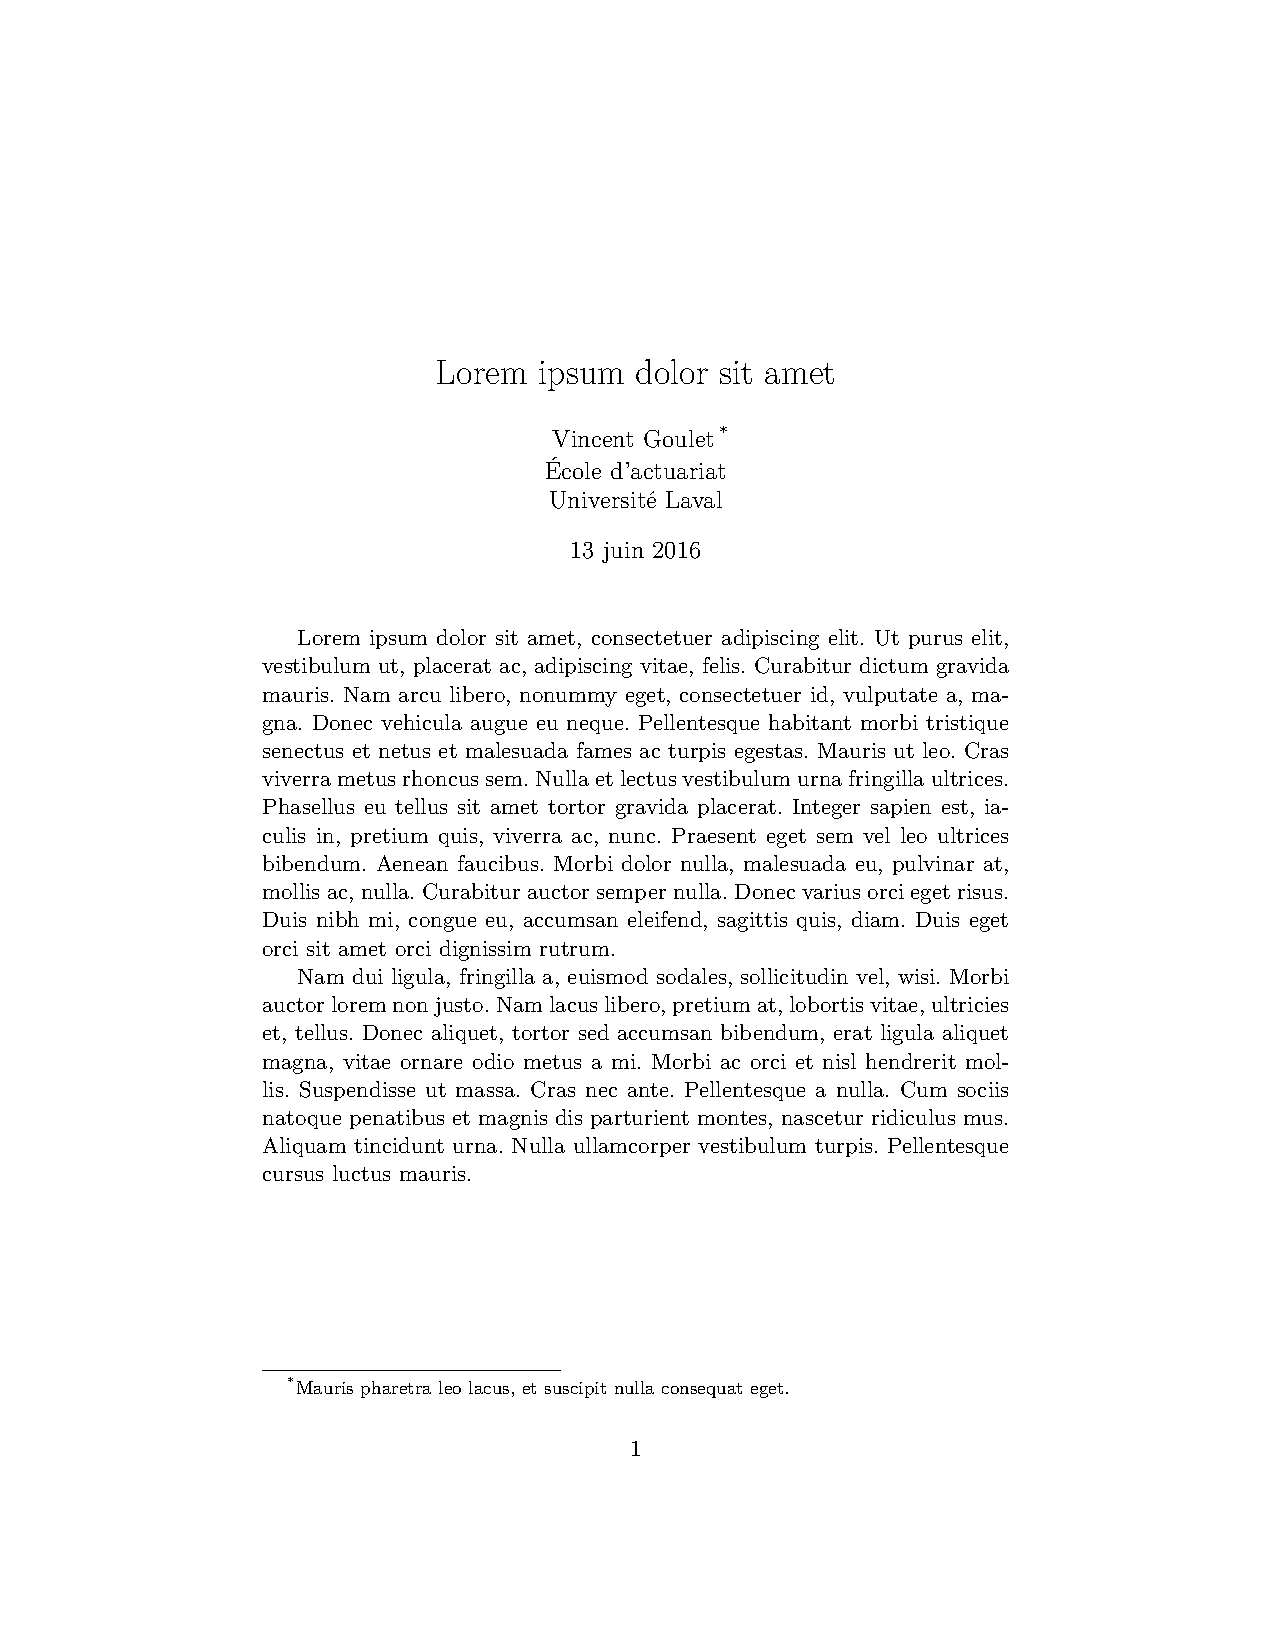
\includegraphics[width=0.7\linewidth]{exemple-titre}}
    \caption{Illustration d'un titre d'article standard.}
    \label{fig:organisation:titre}
  \end{figure}
  \qed
\end{exemple}

Nous avons mentionné plus haut que {\LaTeX} peut aussi produire
automatiquement la page de titre d'un rapport ou d'un livre. Il est
toutefois peu probable qu'elle convienne, surtout dans le cas d'un
livre. Une option plus flexible existe: les environnements
\Ie{titlepage} (classes standards) et \Ie{titlingpage} (classe
\class{memoir}) permettent de définir librement une page de
titre:
\begin{demo}
  \begin{minipage}{0.48\linewidth}
\begin{lstlisting}
\begin{titlepage}
  `\meta{Texte de la page de titre}'
\end{titlepage}
\end{lstlisting}
  \end{minipage}
  \hfill
  \begin{minipage}{0.48\linewidth}
\begin{lstlisting}
\begin{titlingpage}
  `\meta{Texte de la page de titre}'
\end{titlingpage}
\end{lstlisting}
  \end{minipage}
\end{demo}
L'auteur contrôle alors entièrement la disposition et la
composition des éléments de la page de titre. Nous renvoyons le
lecteur au chapitre~4 de la %
\doc{memman}{http://texdoc.net/pkg/memoir} %
de \class{memoir} pour une liste de bonnes pratiques en matière de
composition de page de titre et pour des exemples détaillés.

Comme c'est souvent le cas dans les universités, le format de la page
de titre des thèses et mémoires de l'Université Laval est
prédéterminé. La classe \class{ulthese} fournit donc ses propres
commandes de composition; consulter sa %
\doc{ulthese}{http://texdoc.net/pkg/ulthese}.

\subsection{Résumé}
\label{sec:organisation:parties:resume}

Les articles scientifiques et les rapports comportent souvent un
résumé, habituellement composé en retrait des marges gauche et droite
et dans une police de caractère plus petite. On produit le résumé avec
l'environnement \Ie{abstract} des classes \class{article},
\class{report} ou \class{memoir}:
\begin{lstlisting}
\begin{abstract}
  `\meta{Texte du résumé}'
\end{abstract}
\end{lstlisting}

Il est plutôt rare que les livres comportent un résumé ou alors, comme
d'ailleurs pour les thèses et mémoires de l'Université Laval, celui-ci
est simplement traité comme un chapitre normal non numéroté.

\subsection{Sections}
\label{sec:organisation:parties:sections}

Les commandes ci-dessous servent à découper un document en sections
qui seront automatiquement numérotées par {\LaTeX} de manière
séquentielle:
\begin{lstlisting}
\part`\oarg{titre court}\marg{titre}'
\chapter`\oarg{titre court}\marg{titre}'
\section`\oarg{titre court}\marg{titre}'
\subsection`\oarg{titre court}\marg{titre}'
\subsubsection`\oarg{titre court}\marg{titre}'
\paragraph`\oarg{titre court}\marg{titre}'
\subparagraph`\oarg{titre court}\marg{titre}'
\end{lstlisting}
Les commandes forment, dans l'ordre où elles sont données, une
hiérarchie des titres d'un document\footnote{%
  Nous n'avons jamais utilisé les niveaux de division
  \cmdprint{\paragraph} et \cmdprint{\subparagraph}.}. %
Tel que mentionné précédemment, la commande \cmd{\chapter} n'est pas
disponible avec la classe \class{article}.

Chaque commande prend en argument obligatoire le \meta{titre} de la
section. Si celui-ci est très long, il peut être utile de fournir en
argument optionnel un \meta{titre court}; c'est ce dernier qui
apparaitra dans la table des matières et les entêtes de page, le cas
échéant.

Toutes les commandes existent en version suivie d'une \verb=*= qui
supprime la numérotation ainsi que l'insertion éventuelle dans la
table des matières (plus de détails à la \autoref{sec:organisation:tdm}).

\begin{conseil}
  Éviter d'utiliser des sous-sous-sections numérotées (commande
  \cmdprint{\subsubsection}) dans un livre. Cela résulte en une
  numérotation à quatre niveaux qui s'avère difficile à suivre pour le
  lecteur.
\end{conseil}

\subsection{Annexes}
\label{sec:organisation:parties:annexes}

Les annexes sont des sections ou des chapitres avec une numérotation
alphanumérique (A, A.1, ...) plutôt qu'entièrement numérique. On
informe {\LaTeX} que les sections suivantes doivent être traitées
comme des annexes en insérant dans le document la commande
\begin{lstlisting}
\appendix
\end{lstlisting}
En plus de modifier le style de numérotation, la commande a pour effet
de changer le mot clé «Chapitre» pour «Annexe» dans les titres de
chapitre.

\subsection{Structure logique d'un livre}
\label{sec:oganisation:parties:livre}

Un livre se compose normalement de trois grandes parties logiques: les
pages liminaires (avant-propos, table des matières, tout ce qui
précède le chapitre premier); le corps du livre (chapitres et
annexes); les parties en fin d'ouvrage (bibliographie, index). Les
commandes
\begin{lstlisting}
\frontmatter
\mainmatter
\backmatter
\end{lstlisting}
qui sont disponibles avec les classes \class{book}, \class{memoir} et
\class{ulthese}, permettent d'identifier ces trois parties. Le
\autoref{tab:organisation:livre} résume l'effet de chaque commande.

\begin{table}
  \centering
  \caption{Commandes d'identification de la structure logique d'un
    livre et leurs effets}
  \label{tab:organisation:livre}
  \begin{tabular}{ll}
    \toprule
    Commande & Effets \\
    \midrule
    \cmd{\frontmatter} & numérotation des
                              pages en chiffres romains (i, ii, ...) \\
             & chapitres non numérotés \\
    \addlinespace[0.5\normalbaselineskip]
    \cmd{\mainmatter} & numérotation des pages
                             à partir de 1 en chiffres arabes \\
             & chapitres numérotés \\
    \addlinespace[0.5\normalbaselineskip]
    \cmd{\backmatter} & numérotation des pages
                             se poursuit \\
             & chapitres non numérotés \\
    \bottomrule
  \end{tabular}
\end{table}


\section{Table des matières}
\label{sec:organisation:tdm}

Dans la mesure où l'on a bien identifié les différentes divisions d'un
ouvrage avec les commandes mentionnées à la section précédente, la
production de la table des matières est on ne peut plus simple avec
{\LaTeX}: il suffit d'insérer la commande
\begin{lstlisting}
\tableofcontents
\end{lstlisting}
dans le corps du document à l'endroit où la table des matières doit
apparaître. C'est tout!

Lorsque le paquetage \pkg{hyperref} \citep{hyperref} est chargé, la
commande \cmdprint{\tableofcontents} produit également la table des
matières du fichier PDF. Cela permet de naviguer dans le document
directement depuis la visionneuse PDF. La
\autoref{fig:organisation:tdm-dans-pdf} illustre cette fonctionnalité
avec la visionneuse Aperçu de macOS.

\begin{figure}
  \centering
  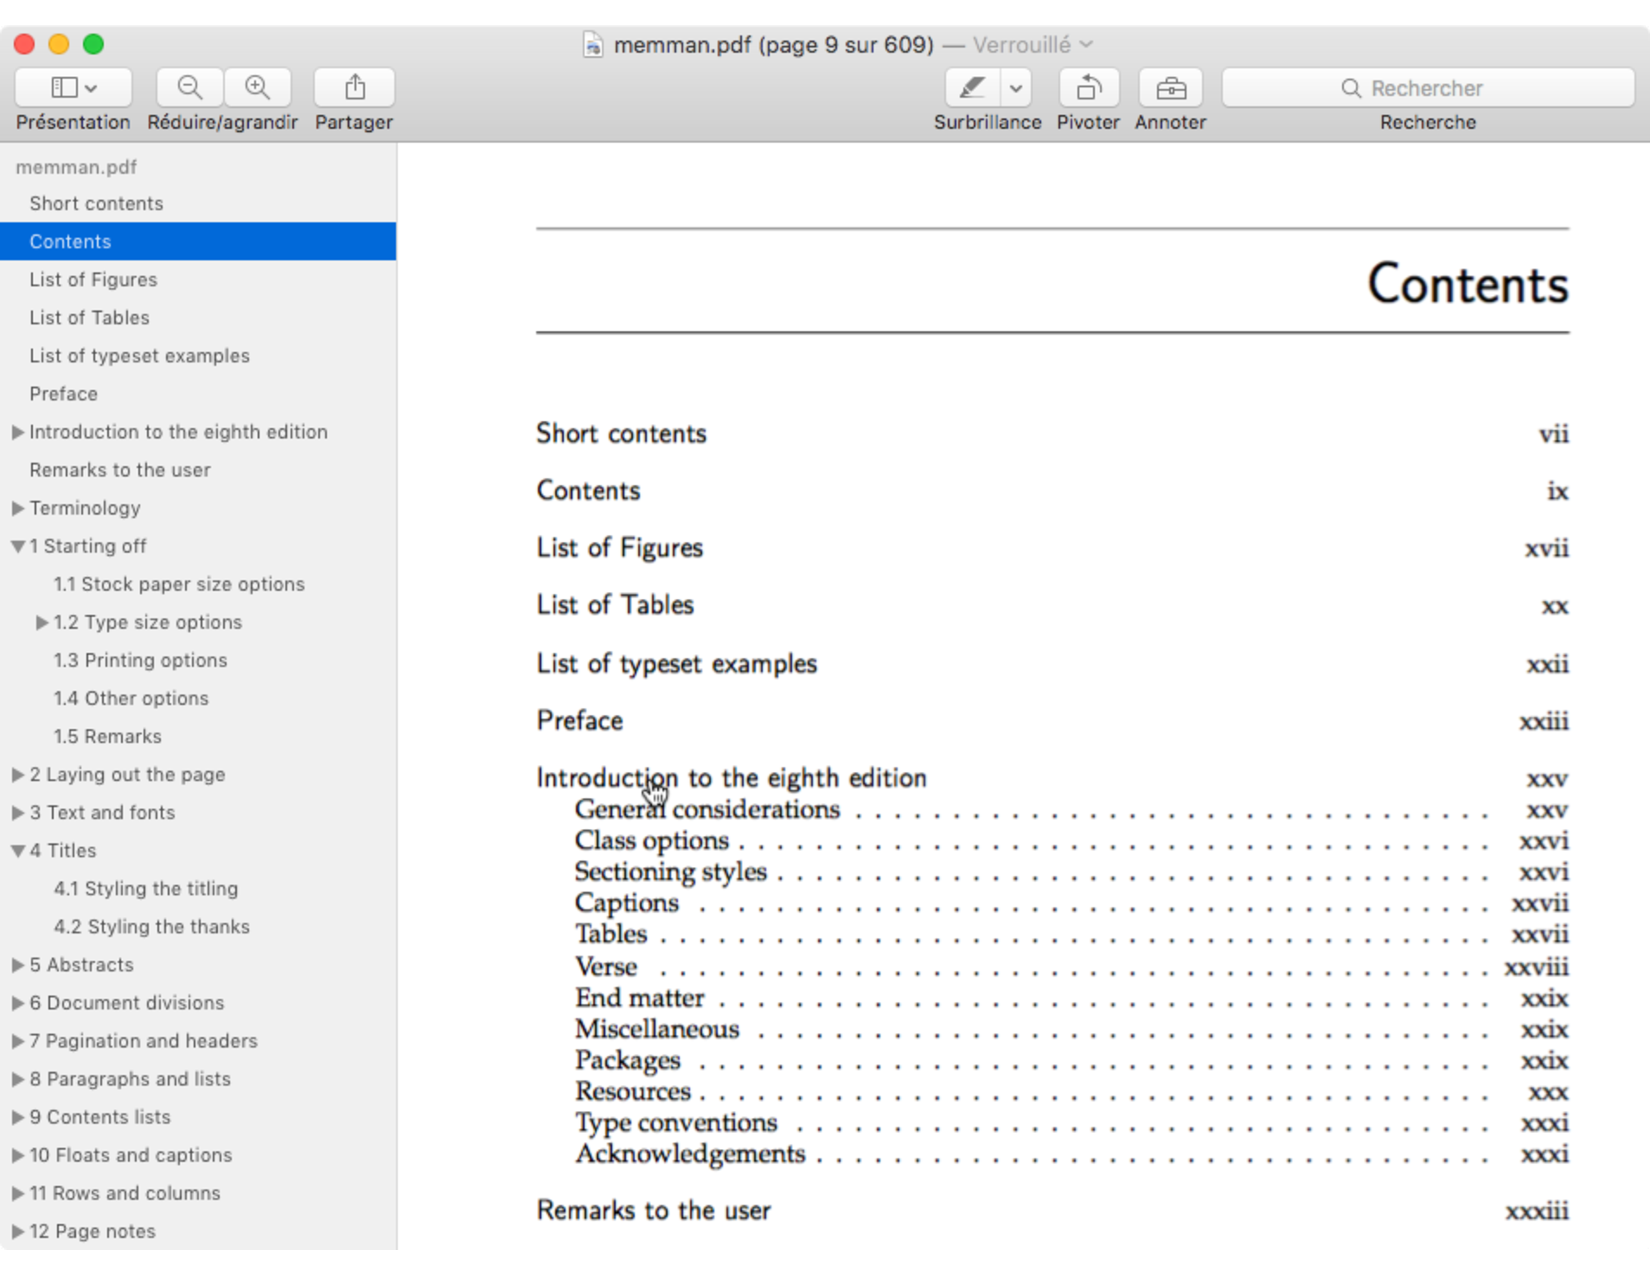
\includegraphics[width=0.7\linewidth,angle=-90]{tdm-dans-pdf}
  \caption{Consultation d'un document PDF avec la visionneuse Aperçu
    de macOS. La barre latérale de gauche affiche la table des
    matières du fichier PDF, ce qui permet de naviguer dans le
    document sans devoir revenir à celle du document.}
  \label{fig:organisation:tdm-dans-pdf}
\end{figure}

\begin{important}
  La production initiale de la table des matières et la prise en
  compte de toute modification requiert jusqu'à trois compilations
  consécutives du document.
\end{important}

Par défaut, une section non numérotée ne figure pas dans la table des
matières. Si l'on souhaite néanmoins l'y insérer, il faut utiliser la
commande suivante:
\begin{lstlisting}
\addtocontentsline{toc}`\marg{niveau}\marg{titre}'
\end{lstlisting}
où \meta{niveau} est le nom de la commande de division sans le
caractère {\bs} (\code{chapter}, \code{section}, etc.) et \meta{titre}
est le texte qui apparaitra dans la table des matières.

\begin{exemple}
  Selon les normes de présentation visuelle de la Faculté des études
  supérieures et postdoctorales pour les thèses et mémoires de
  l'Université Laval, les résumés, la liste des abbréviations et des
  sigles, les remerciements et l'avant-propos doivent être composés
  comme des chapitres normaux non numérotés. Cependant, ils doivent
  apparaître dans la table des matières. Pour ce faire, les gabarits
  fournis avec la classe \class{ulthese} comportent des lignes de la
  forme:
\begin{lstlisting}
\chapter*{Résumé}
\phantomsection\addcontentsline{toc}{chapter}{Résumé}
\end{lstlisting}
  La commande \cmd{\phantomsection} est rendue nécessaire (ou
  recommandée) par le paquetage \pkg{hyperref}. %
  \qed
\end{exemple}

Outre une table des matières, les longs ouvrages scientifiques
comptent parfois une liste des figures et une liste des tableaux. On
obtient celles-ci avec les commandes
\begin{lstlisting}
\listoffigures
\listoftables
\end{lstlisting}

Dans les classes \class{memoir} et \class{ulthese}, les commandes
ci-dessus insèrent leur propre titre de section dans la table des
matière (autrement dit, la table des matières apparait dans la table
des matières). Les versions
\begin{lstlisting}
\tableofcontents*
\listoffigures*
\listoftables*
\end{lstlisting}
adoptent le comportement des classes standards, soit d'omettre ces
parties dans la table des matières.


\section{Renvois automatiques}
\label{sec:construction:renvois}


\subsection{Étiquettes et renvois}

Parce que l'ordinateur le fera mieux que vous

\begin{itemize}
\item Ne \emph{jamais} renvoyer manuellement à un numéro de section,
  d'équation, de tableau, etc.
\item «Nommer» un élément avec \verb=\label=
\item Faire référence par son nom avec \verb=\ref=
\item Requiert 2 à 3 compilations
\end{itemize}

\begin{demo}
\begin{lstlisting}[emph={\label,\ref}]
\section{Définitions}
\label{sec:definitions}

Lorem ipsum dolor sit amet, consectetur
adipiscing elit. Duis in auctor dui. Vestibulum

\section{Historique}

Tel que vu à la section \ref{sec:definitions},
on a...
\end{lstlisting}
  \begin{framed}
    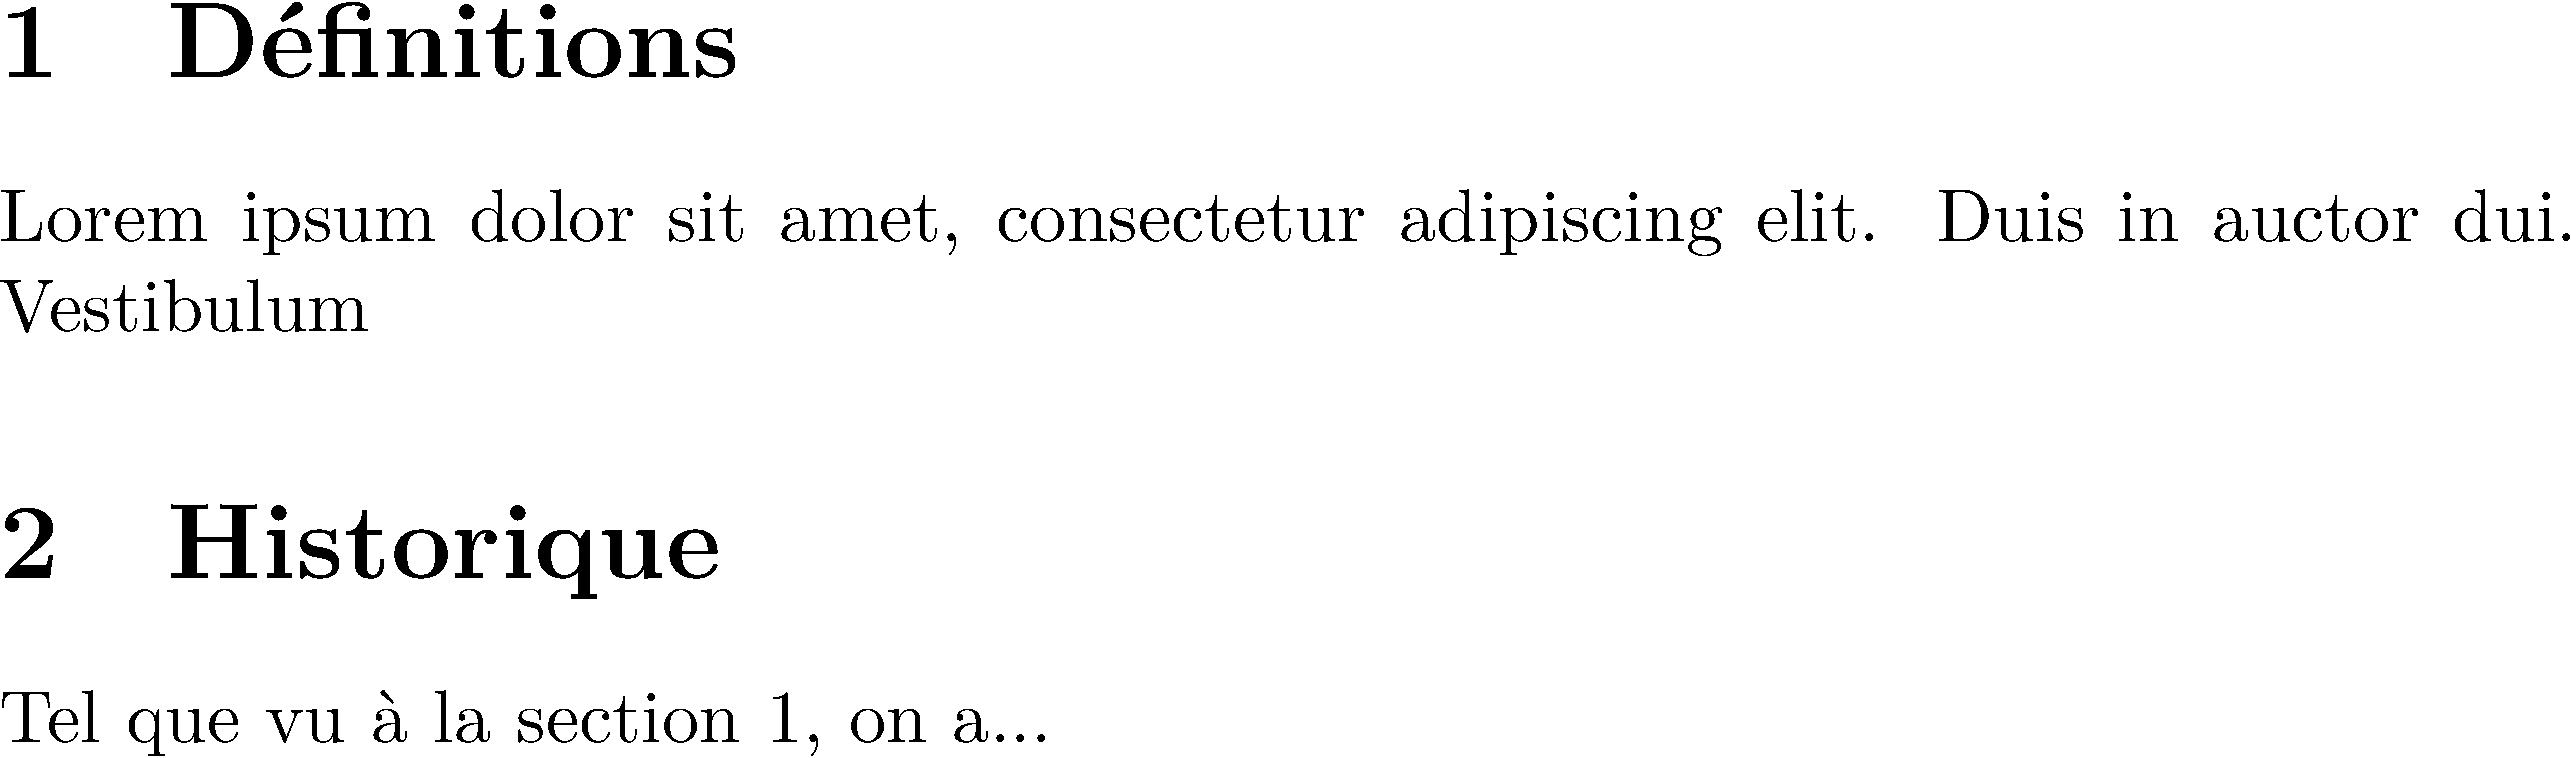
\includegraphics[width=\linewidth]{renvoi}
  \end{framed}
\end{demo}

\begin{conseil}
  Adoptez une manière systématique et mnémotechnique de nommer les
  éléments dans un long document afin de vous y retrouver.

  \bigskip %
  Exemple:
\begin{lstlisting}
\label{chap:`\meta{chapitre}'}          % chapitre
\label{sec:`\meta{chapitre}':`\meta{section}'}  % section
\label{tab:`\meta{chapitre}':`\meta{tableau}'}  % tableau
\label{eq:`\meta{chapitre}':`\meta{equation}'}  % équation
\end{lstlisting}
\end{conseil}


\subsection{Hyperliens}

Renvois automatiques++

\begin{itemize}
\item Paquetage \pkg{hyperref} insère des hyperliens vers les renvois
  dans les fichiers PDF
  \begin{demo}
\begin{lstlisting}
Tel que vu à la section \ref{sec:definitions},
on a...
\end{lstlisting}
    \begin{framed}
      
\includegraphics{renvoi_avec_ref}
    \end{framed}
  \end{demo}
\item Commande \verb=\autoref= permet de
  \begin{enumerate}
  \item nommer automatiquement le type de renvoi (section, équation,
    tableau, etc.)
  \item transformer en hyperlien le texte \textbf{et} le numéro
  \end{enumerate}
  \begin{demo}
\begin{lstlisting}
Tel que vu à la \autoref{sec:definitions},
on a...
\end{lstlisting}
    \begin{framed}
      
\includegraphics{renvoi_avec_autoref}
    \end{framed}
  \end{demo}
\end{itemize}




%%%
%%% Exercices
%%%

\section{Exercices}
\label{sec:apparence:exercices}

\begin{exercice}[nosol]
  Utiliser le fichier \fichier{exercice\_parties.tex}.
  \begin{enumerate}
  \item Étudier la structure du document dans le code source.
  \item Ajouter un titre et un auteur au document.
  \item Créer la table des matières du document en le compilant 2 à 3
    fois.
  \item Insérer deux ou trois titres de sections de différents niveaux
    dans le document.
  \item Vous remarquerez que la numérotation cesse à partir des
    sous-sections. C'est une particularité de la classe
    \class{memoir}.

    Recompiler le document après avoir ajouté au préambule la commande
\begin{lstlisting}
\maxsecnumdepth{subsection}
\end{lstlisting}
  \item Ajouter une annexe au document.
  \end{enumerate}
\end{exercice}

\begin{exercice}[nosol]
  Utiliser le fichier \fichier{exercice\_renvois.tex}.
  \begin{enumerate}
  \item Insérer dans le texte un renvoi au numéro d'une section.
  \item Activer le paquetage \pkg{hyperref} avec l'option
    \code{colorlinks} et comparer l'effet d'utiliser \cmd{\ref} ou
    \cmd{\autoref} pour le renvoi.
  \end{enumerate}
\end{exercice}


%%% Local Variables:
%%% mode: latex
%%% TeX-engine: xetex
%%% TeX-master: "formation-latex-ul"
%%% coding: utf-8
%%% End:
